\section{Illustration of Effectively Sampled Arms by \texorpdfstring{\DTTTS}{}}\label{app:dttts.arms}

One drawback of the current \DTTTS is that it may not work well if we do not know the oracle $\mu^\star$ ($\mu^\star$ is set to 1 in our previous experiments). Fig.~\ref{fig:shift} shows the expected simple regret of \DTTTS compared to \ISHA and \TTTS under a $\texttt{Beta}(0.5,0.5)$ reservoir shifted by 0.8, 0.6, 0.4, 0.2 and without shift respectively. A Beta distribution $\texttt{Beta}(a,b)$ shifted by $\mu^\star$ is obtained by re-scaling to $[0,\mu^*]$ the corresponding distribution. More formally, a shifted Beta distribution on $[0,\mu^*]$, denoted by  $\texttt{SB}_{\mu^\star}(a,b)$ in the rest of the paper, is the distribution of $X\mu^*$ where $X \sim \texttt{Beta}(a,b)$ (see Appendix~\ref{app:dttts.adapt} for more discussion on shifted Beta distributions). We can see that the performance of \DTTTS is getting worse along with the increasing shift.

\begin{figure}[ht]
  \centering
  \begin{subfigure}[ht]{0.33\textwidth}
    \centering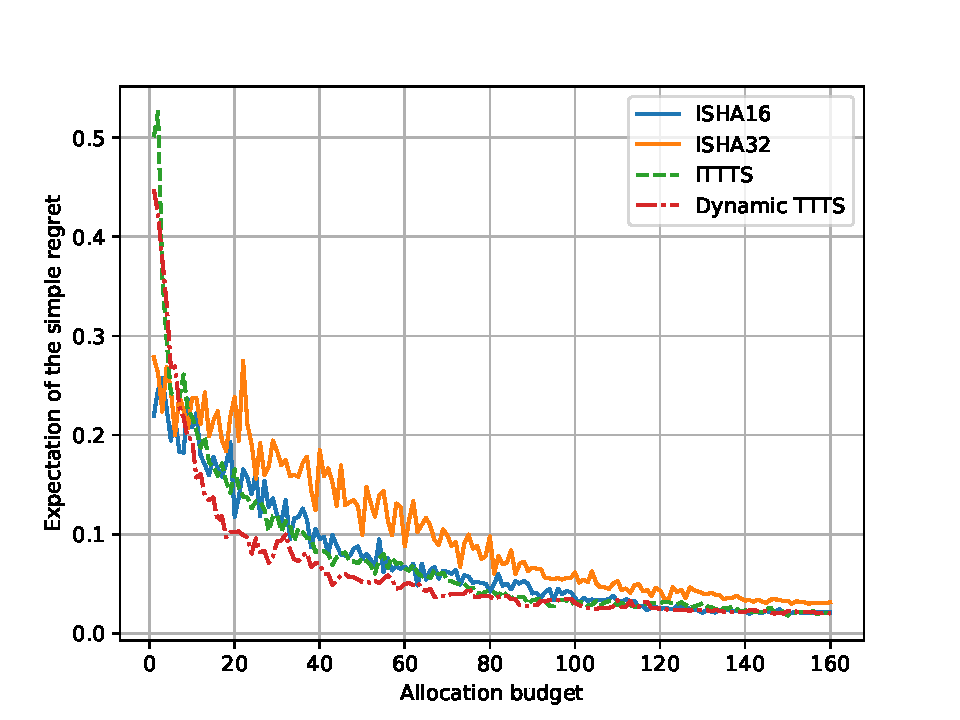
\includegraphics[width=\textwidth]{Chapter6/img/shift/no_shift.pdf}
    \caption{no shift}
  \end{subfigure}%
  \begin{subfigure}[ht]{0.33\textwidth}
    \centering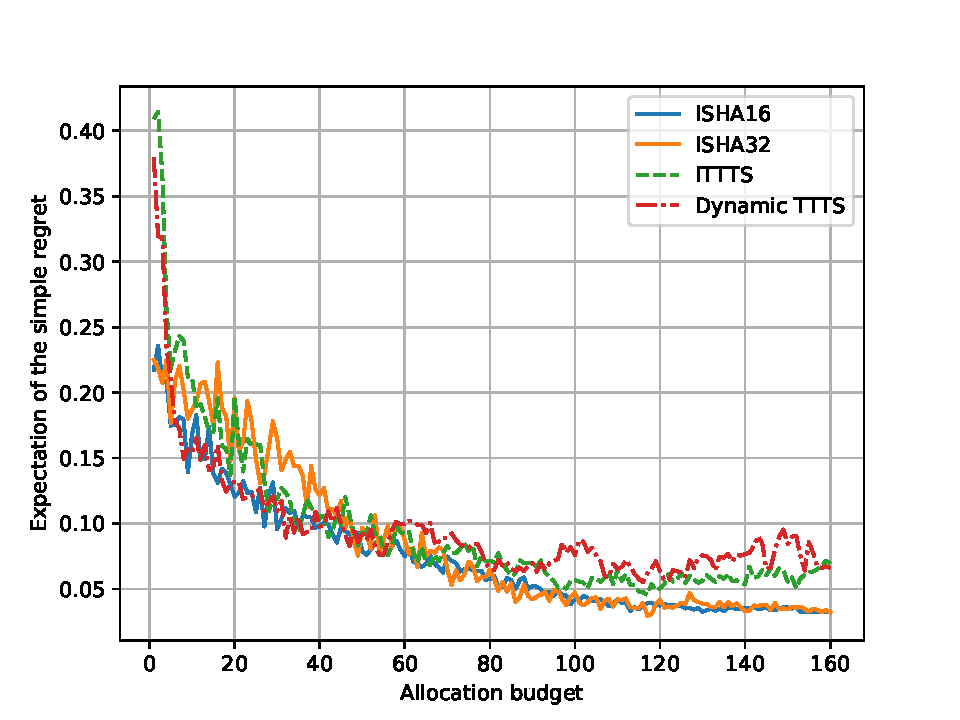
\includegraphics[width=\textwidth]{Chapter6/img/shift/shift_-8.pdf}
    \caption{shift by 0.8}
  \end{subfigure}
    \begin{subfigure}[ht]{0.33\textwidth}
    \centering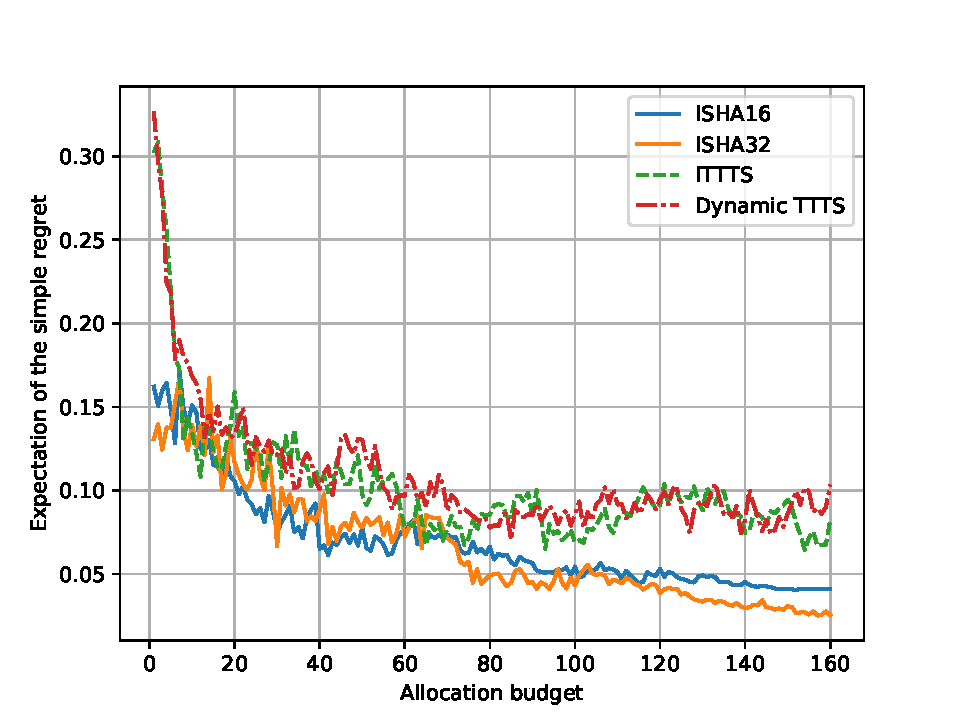
\includegraphics[width=\textwidth]{Chapter6/img/shift/shift_-6.pdf}
    \caption{shift by 0.6}
  \end{subfigure}%
  \begin{subfigure}[ht]{0.33\textwidth}
    \centering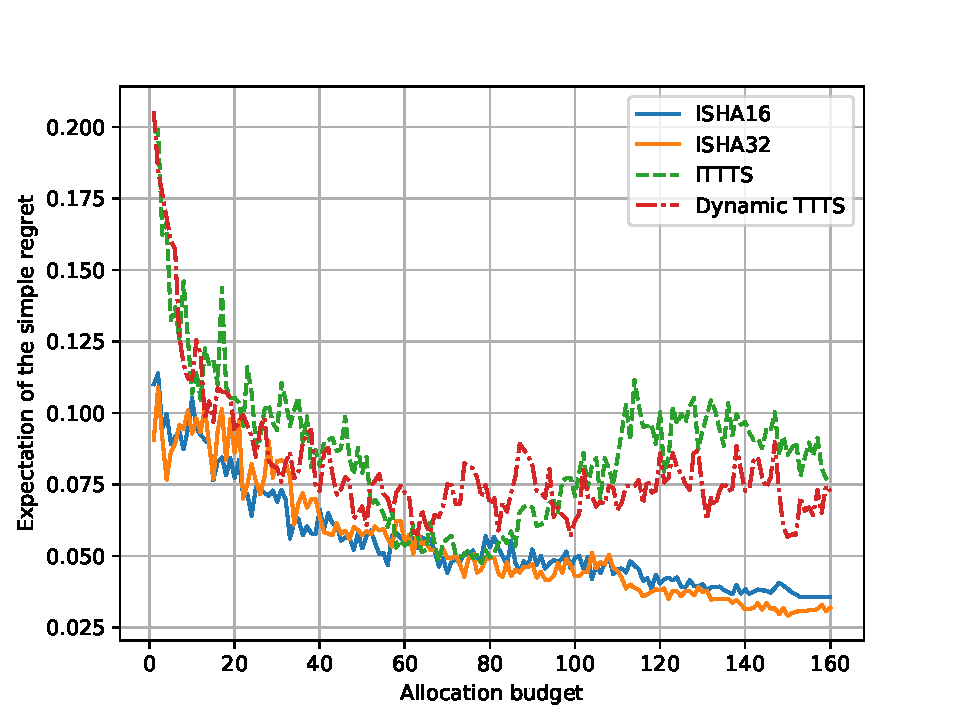
\includegraphics[width=\textwidth]{Chapter6/img/shift/shift_-4.pdf}
    \caption{shift by 0.4}
  \end{subfigure}
  \begin{subfigure}[ht]{0.33\textwidth}
    \centering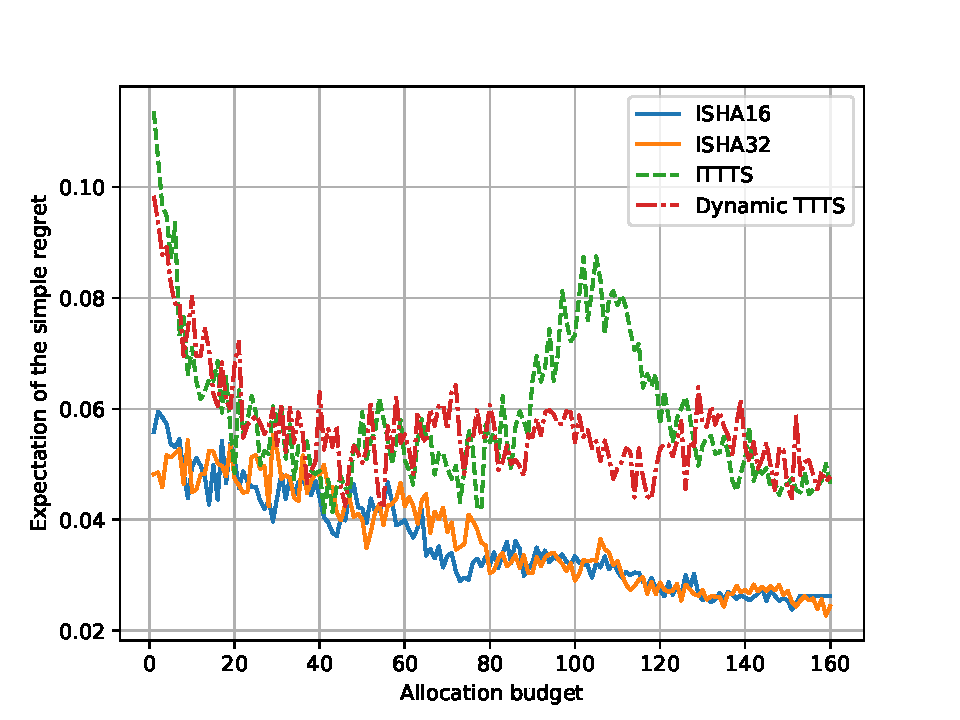
\includegraphics[width=\textwidth]{Chapter6/img/shift/shift_-2.pdf}
    \caption{shift by 0.2}
  \end{subfigure}%
  \caption{Simple regret of \DTTTS (against \Hyperband) for shifted Beta reservoir.}
  \label{fig:shift}
\end{figure}

As suggested by the implementation trick introduced in Section~\ref{sec:dttts.algorithm}, all the $k$ arms that have been added but not effectively sampled can be seen as a virtual arm endowed with a $\texttt{Beta}(k,1)$ posterior. Intuitively, if $\mu^\star < 1$, than this virtual arm would force the algorithm to sample too many new arms, thus would lack of attention on arms that are more likely to be near-optimal. This intuition is supported by the illustration in Fig.\,\ref{fig:shifted_reservoir}: the posterior distributions of effectively sampled will eventually be supported mostly on the left of $\mu^*$, while the pseudo-arm still put a lot of mass near 1. 

In Fig.\,\ref{fig:arms_shift}, we report the number of arms that have been played $1,2,\dots,9$ and more than $10$ times for \DTTTS run under a $\texttt{Beta}(0.5,0.5)$, $\texttt{SB}_{0.8}(0.5,0.5)$, $\texttt{SB}_{0.6}(0.5,0.5)$, $\texttt{SB}_{0.4}(0.5,0.5)$ and $\texttt{SB}_{0.2}(0.5,0.5)$ reservoir respectively, which confirms the over-exploration effect caused by shifted reservoirs.

\begin{figure}[ht]
  \centering
  \begin{subfigure}[ht]{0.45\textwidth}
    \centering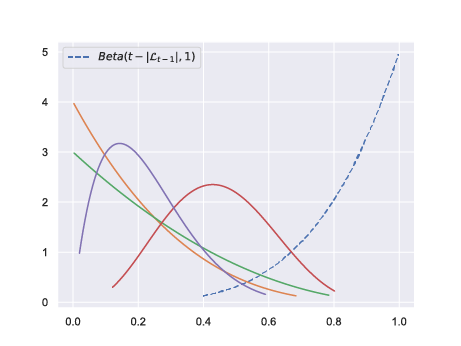
\includegraphics[width=\textwidth]{Chapter6/img/shift/order_trick.png}
    \caption{posterior distributions of the effectively samples arms and the pseudo-arm}
    \label{fig:shifted_reservoir}
  \end{subfigure}%
  \hspace{0.5cm}
  \begin{subfigure}[ht]{0.45\textwidth}
    \centering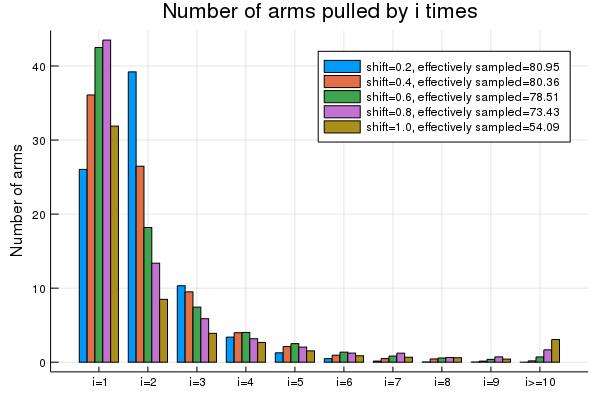
\includegraphics[width=\textwidth]{Chapter6/img/infinite/pulls_shift.png}
    \caption{number of effectively sampled arms, averaged over 100 runs}
    \label{fig:arms_shift}
  \end{subfigure}%
  \caption{Illustration of over-exploration of \DTTTS under shifted reservoirs.}
  \label{fig:arms}
\end{figure}

In the next section, we propose a simple fix for the algorithm that is not tailored for $\mu^*=1$ but adjusts to any value of $\mu^*$.
